% !TEX root = ../main.tex
    \begin{figure}[b!]
        \frame{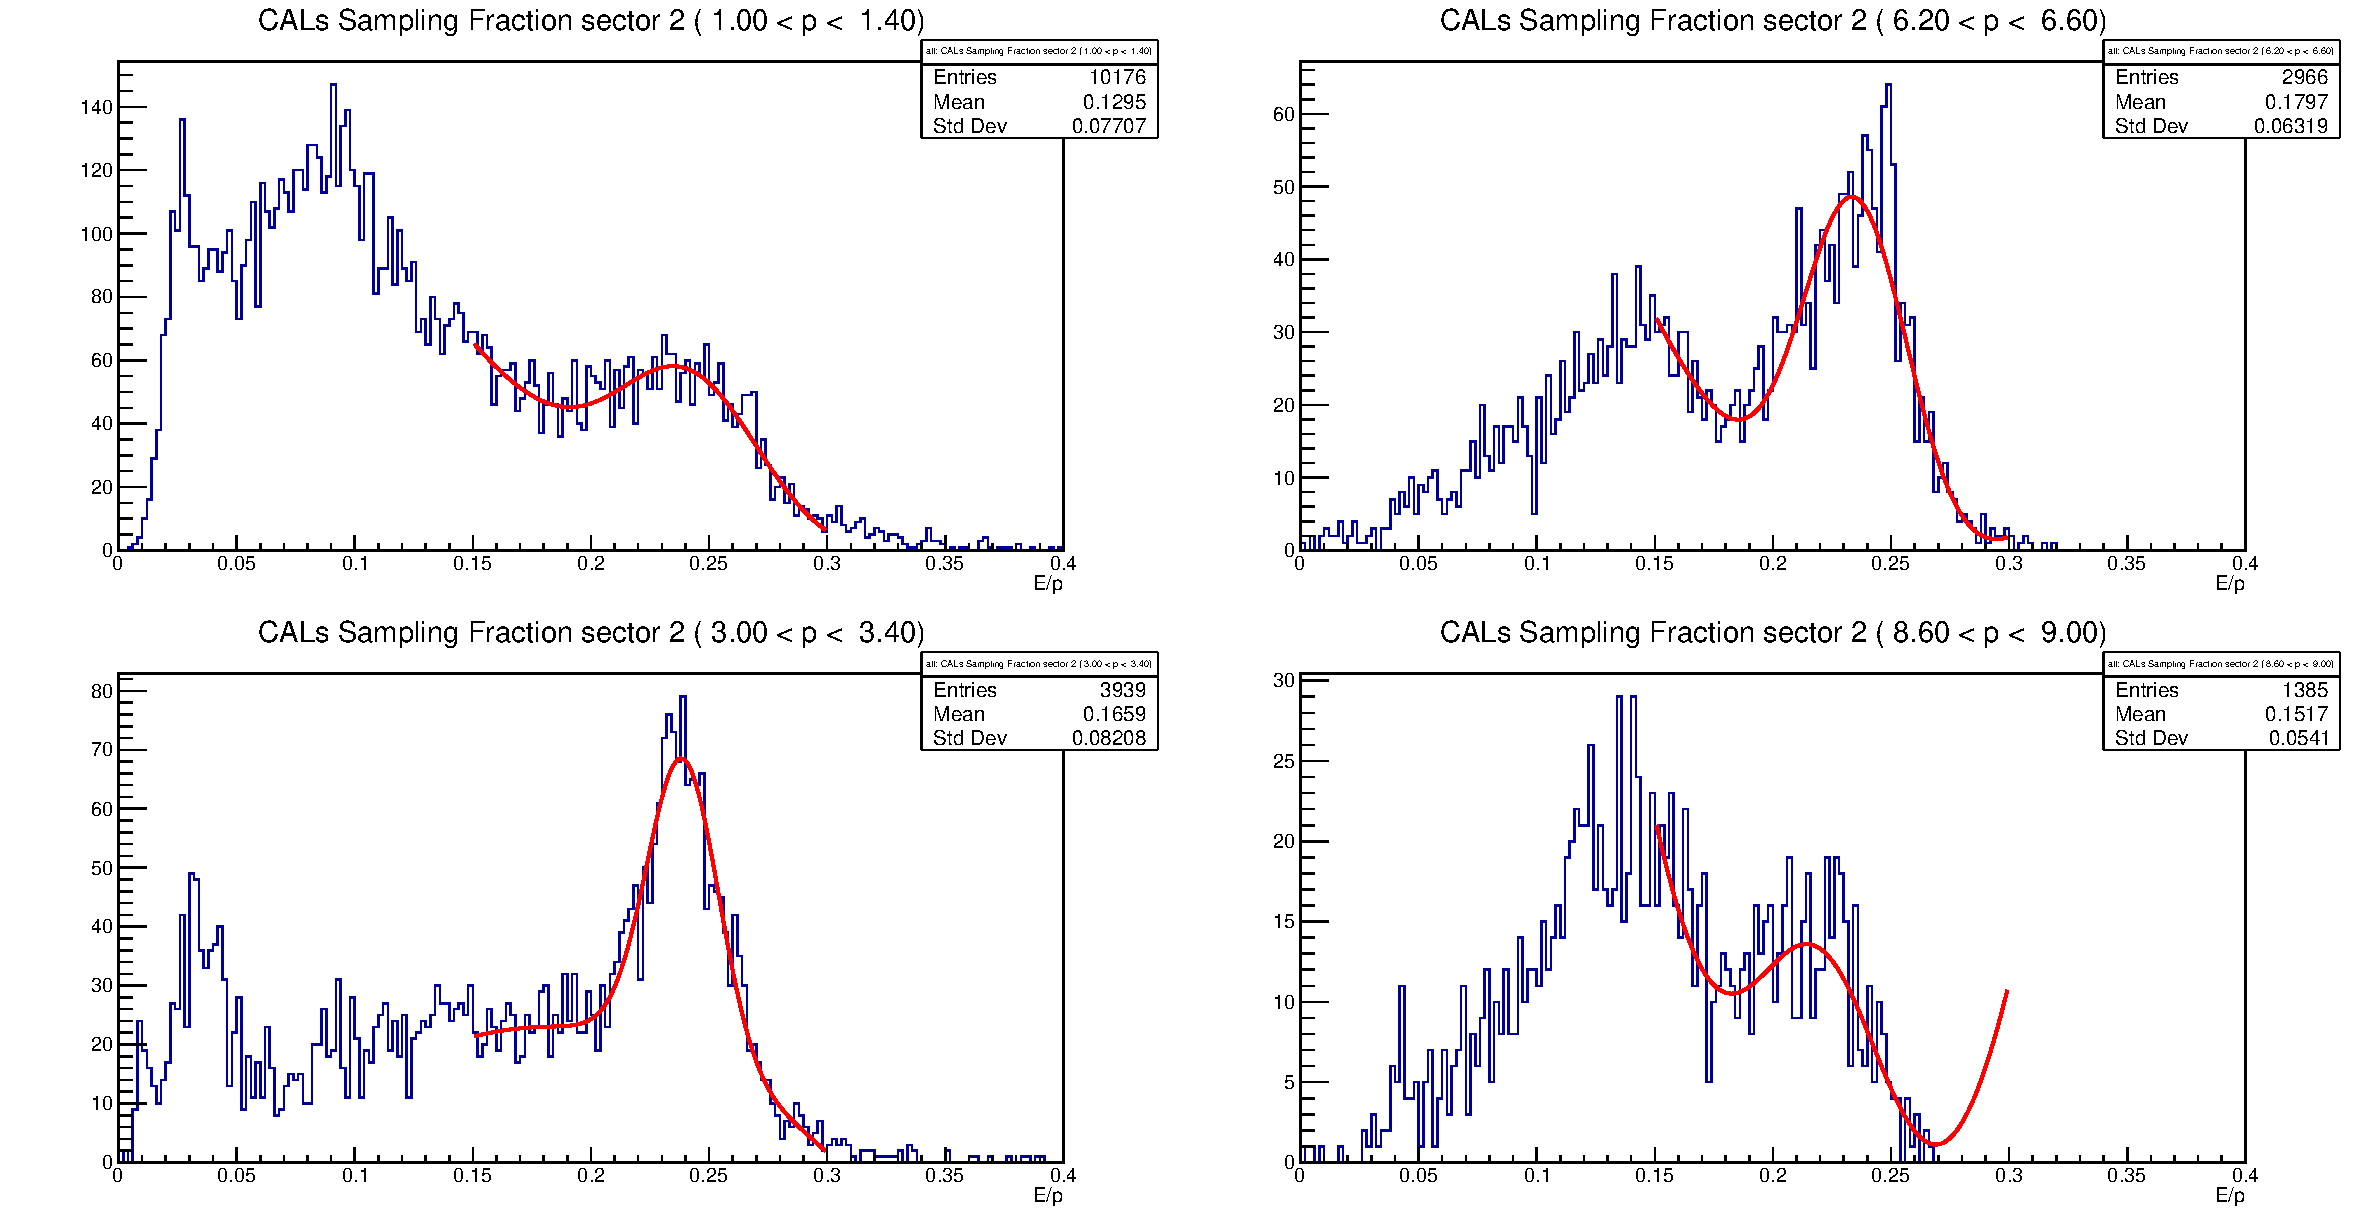
\includegraphics[width=\textwidth]{30sf_1d_plots.pdf}}
        \caption[Calorimeters $E/p$ plots]
        {Four $E/p$ plots describing the sum of the deposited energy per particle on all calorimeters (PCAL, ECIN, and ECOU).
        The particles' momentum is obtained from tracking and the event builder.
        As can be seen in the northwest and the southeast plots, the corner bins -- $1.00$ to $1.40$ and $8.60$ to $9.00$ GeV respectively -- are not very reliable.}
        \floatfoot{Source: Own elaboration, using the \href{https://github.com/bleaktwig/clas12-rge-analysis}{clas12-rge-analysis} software.}
        \label{fig::13.30::sampling_fraction_fit_1d}
    \end{figure}

\subsection{Sampling Fraction}
\label{13.30::sampling_fraction}
    The energy deposited by electrons in the active area of the calorimeters is a fraction of their total energy, $E_\text{tot}$.
    This value is proportional to their momentum, $P$, for energies above a few hundred MeV.
    Heavier particles, due to their reduced penetration capabilities, tend to lose an amount of energy independent of their momentum.
    The electron sampling fraction measures the amount of energy lost depending on the momentum of a particle.
    This allows for both the measurement of the electron's energy and the differentiation of electrons from other particles \cite{wigmans2000}.

    To obtain the sampling fraction, the hits of each calorimeter by itself (PCAL, ECIN, and ECOU) are separated into arrays, with an additional array containing the union of the other three.
    Then, these arrays of hits are separated into 20 momentum bins.
    Each bin has a size of 0.4 GeV, starting at 1.0 GeV and ending at 9.0 GeV.

    1-dimensional histograms are then created from the data in these arrays, measuring the deposited energy divided by the vertex momentum ($E/p$).
    A Gaussian fit plus a quadratic background is then applied, following the function described as

    \begin{equation*}
        f(x) = p_0 g(x, \mu, \sigma) + p_1 x^2 + p_2 x + p_3, \hspace{12pt}
        \text{where} \hspace{4pt}
        g(x, \mu, \sigma) = \frac{1}{\sigma \sqrt{2\pi}} \exp \left(-\frac{1}{2} \frac{(x - \mu)^2}{\sigma^2}\right),
    \end{equation*}

    where $\mu$ and $\sigma$ represent the mean and standard deviation of the distribution, respectively. The fit is limited to the range between $0.15$ and $0.30$ for the expected $E/p$ values for electrons based on theory.

    Examples of these plots are shown in Figure \ref{fig::13.30::sampling_fraction_fit_1d}.
    From the figure, it can be observed that there are not enough electrons in the extreme momentum ranges, such as from $1$ to $1.4$ GeV or from $8.6$ to $9$ GeV.
    Consequently, the sampling fraction fit, described in Equation \eqref{eq::13.30::sampling_fraction_fit_2d}, only considers data within the range of $1.4$ to $8.6$ GeV.

    The mean of each of these fits is then extracted to serve as data points for a sampling fraction fit.
    A polynomial fit is employed since it effectively captures the shape of these points and aligns with the reconstruction software.
    The fit is described as

    \begin{equation} \label{eq::13.30::sampling_fraction_fit_2d}
        f(x) = p_0 \cdot \left(p_1 + \frac{p_2}{x} + \frac{p_3}{x^2}\right).
    \end{equation}

    The $E/p$ distribution vs $p$ is depicted in Figure \ref{fig::13.30::sampling_fraction_fit_2d}, together with this fit.

    \begin{figure}[t!]
        \frame{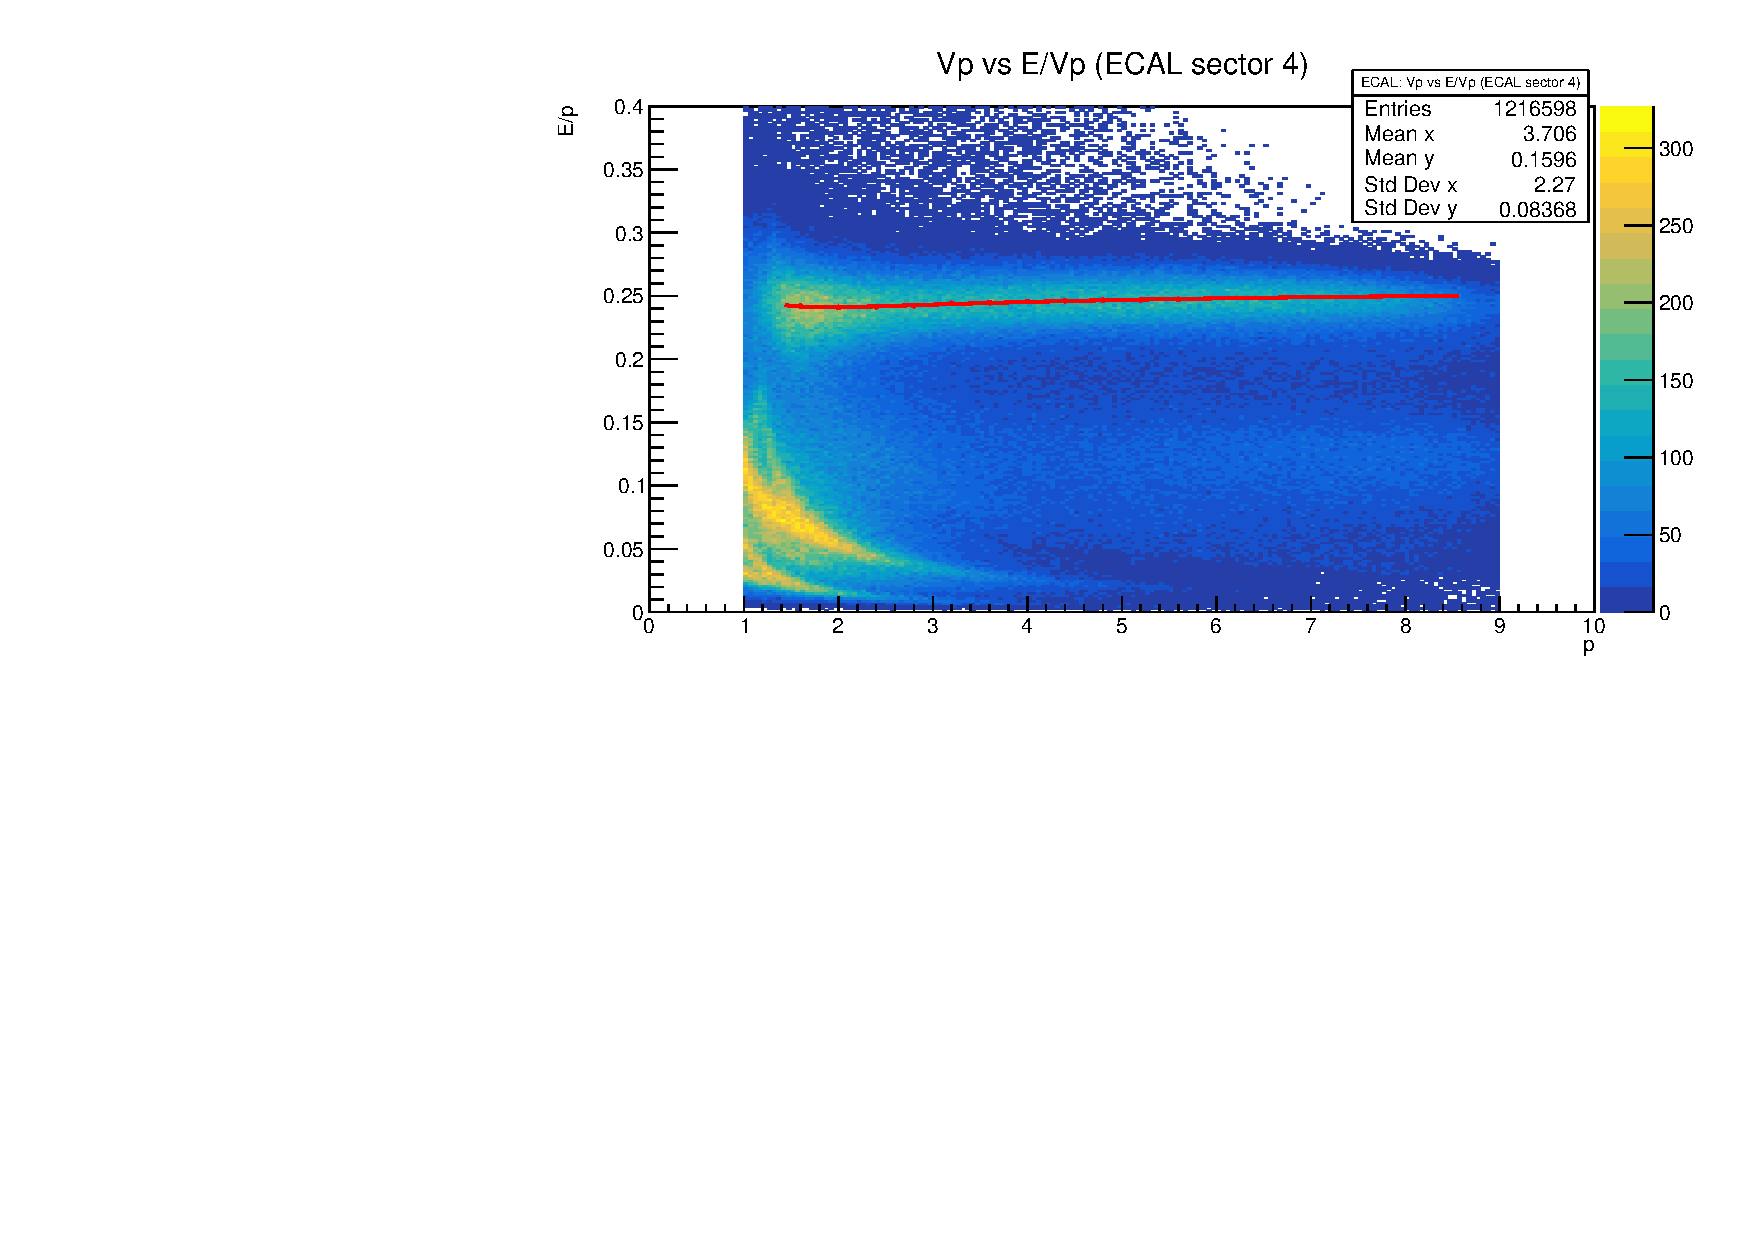
\includegraphics[width=\textwidth]{30sf_2d_plot.pdf}}
        \caption[Calorimeters $p vs E/p$ plots]
        {A 2D plot showing momentum $p$ vs deposited energy divided by momentum $E/p$.
        The particle's deposited energy on all calorimeters is measured.
        Its momentum is obtained from tracking and the event builder.
        The fit follows the deposited energy of electrons to find their sampling fraction.}
        \floatfoot{Source: Own elaboration, using the \href{https://github.com/bleaktwig/clas12-rge-analysis}{clas12-rge-analysis} software.}
        \label{fig::13.30::sampling_fraction_fit_2d}
    \end{figure}

    Finally, the parameters of the fit are saved in plain text files, following the convention used in the CCDB.
    These parameters can be utilised later for particle identification purposes, specifically for electrons and photons.
    Furthermore, they are employed to determine the energy of electrons and photons since, as mentioned previously, not all of their energy is deposited in the calorimeters.
